%Template
% !TeX spellcheck = de 
\documentclass[a4paper]{scrartcl}
\usepackage[utf8]{inputenc}
%\usepackage[ngerman]{babel}
\usepackage{geometry,forloop,fancyhdr,fancybox,lastpage}
\usepackage{listings}
\lstset{frame=tb,
	language=Java,
	aboveskip=3mm,
	belowskip=3mm,
	showstringspaces=false,
	columns=flexible,
	basicstyle={\small\ttfamily},
	numbers=left,
	numberstyle=\tiny\color{gray},
	keywordstyle=\color{blue},
	commentstyle=\color{dkgreen},
	stringstyle=\color{mauve},
	breaklines=true,
	breakatwhitespace=true,
	tabsize=3
}
\geometry{a4paper,left=3cm, right=3cm, top=3cm, bottom=3cm}
% Diese Daten müssen pro Blatt angepasst werden:
\newcommand{\NUMBER}{2}
\newcommand{\EXERCISES}{4}
% Diese Daten müssen einmalig pro Vorlesung angepasst werden:
\newcommand{\COURSE}{Einführung in Maschinelles Lernen}
\newcommand{\TUTOR}{TBD}
\newcommand{\STUDENTA}{Maria Heitmeier}
\newcommand{\STUDENTB}{Gwent Krause}
\newcommand{\STUDENTC}{Stefan Wezel}
\newcommand{\DEADLINE}{23.05.2018}




%Math
\usepackage{amsmath,amssymb,tabularx}

%Figures
\usepackage{graphicx,tikz,color,float}
\graphicspath{ {home/stefan/picures/} }
\usetikzlibrary{shapes,trees}

%Algorithms
\usepackage[ruled,linesnumbered]{algorithm2e}

%Kopf- und Fußzeile
\pagestyle {fancy}
\fancyhead[L]{\COURSE}
\fancyhead[C]{\STUDENTA, \STUDENTB, \STUDENTC\\}
\fancyhead[R]{\today}

\fancyfoot[L]{}
\fancyfoot[C]{}
\fancyfoot[R]{Seite \thepage}

%Formatierung der Überschrift, hier nichts ändern
\def\header#1#2{
	\begin{center}
		{\Large\bf Übungsblatt #1}\\
		{(Abgabetermin #2)}
	\end{center}
}

%Definition der Punktetabelle, hier nichts ändern
\newcounter{punktelistectr}
\newcounter{punkte}
\newcommand{\punkteliste}[2]{%
	\setcounter{punkte}{#2}%
	\addtocounter{punkte}{-#1}%
	\stepcounter{punkte}%<-- also punkte = m-n+1 = Anzahl Spalten[1]
	\begin{center}%
		\begin{tabularx}{\linewidth}[]{@{}*{\thepunkte}{>{\centering\arraybackslash} X|}@{}>{\centering\arraybackslash}X}
			\forloop{punktelistectr}{#1}{\value{punktelistectr} < #2 } %
			{%
				\thepunktelistectr &
			}
			#2 &  $\Sigma$ \\
			\hline
			\forloop{punktelistectr}{#1}{\value{punktelistectr} < #2 } %
			{%
				&	
			} &\\
			\forloop{punktelistectr}{#1}{\value{punktelistectr} < #2 } %
			{%
				&
			} &\\
		\end{tabularx}
	\end{center}
}

\begin{document}
	
\section*{Aufgabe 1}
<<<<<<< HEAD
\begin{itemize}
	\item[a)] Der Satz von Bayes:\\ \ \\
	$prob(A|B) = \frac{prob(B|A) \cdot prob(A)}{prob(B)}$\\
	\ \\
	prob(B$|$A) ist die likelihood, prob(A) die A-Priori-Wahrscheinlichkeit fuer die Hypothese, prob(B) die A-Priori-Wahrscheinlichkeit fuer die Daten und das Ergebnis ist die A-Posteriori-Wahrscheinlichkeit.\\
	\ \\
	Bei der Klassifizierung von Barschen und Lachsen wird damit bestimmt wie wahrscheinlich es ist, dass anhand der Wahrscheinlichkeit der Laenge und dass es ein Lachs ist, dass sich um die Lachs handelt. 
=======
>>>>>>> 1c3819657581e0d05b08f7d499fe85dea81efea6

	\subsection*{a)} Sei H eine Hypothese und D Daten. Dann lautet der Satz von Bayes: $$p(H|D) = \frac{p(D|H)p(H)}{p(D)}$$
	Die einzelnen Terme werden im Folgenden anhand des Beispiel der Berechnung der Masse des Saturns erklärt.\\
	$p(D|H)$ ist die likelihood, also die Wahrscheinlichkeit für die Daten, gegeben die Hypothese. Das bedeutet im Beispiel, wie wahrscheinlich ist es, dass diese Daten auftreten und die Hypothese, dass der Saturn eine bestimmte Masse hat.\\
	$p(H)$ ist die A-priori-Wahrscheinlichkeit, also die Wk, dass die Hypothese stimmt. Die Wk dafür, dass der Saturn die gegebene Masse hat.\\
	$p(D)$ ist die evidence, die Wk, die gegebenen Daten zu beobachten. Wie wahrscheinlich ist es, beim Saturn eine bestimmte Masse zu beobachten.\\
	$p(H|D)$ nennt man die A-posteriori-Wahrscheinlichkeit, also die Wk, dass die Hypothese stimmt, gegeben die Daten. Die Wahrscheinlichkeit, dass der Saturn tatsächlich die gegebene Masse hat, gegeben die beobachteten Daten.

	%\item[a)] Der Satz von Bayes:\\ \ \\
	%$prob(A|B) = \frac{prob(B|A) \cdot prob(A)}{prob(B)}$\\
	%\ \\
	%prob(B|A) ist die likelihood, prob(A) die A-Priori-Wahrscheinlichkeit fuer die Hypothese, prob(B) die A-Priori-Wahrscheinlichkeit fuer die Daten und das Ergebnis ist die A-Posteriori-Wahrscheinlichkeit.\\
	%\ \\
	%Bei der Klassifizierung von Barschen und Lachsen wird damit bestimmt wie wahrscheinlich es ist, dass anhand der Wahrscheinlichkeit der Laenge und dass es ein Lachs ist, dass sich um die Lachs handelt. 
%\end{itemize}

\subsection*{b)}













\item[(c)]
Mithilfe der Bayes'schen Entscheidungsregel können zwischen zwei Hypothesen unterscheiden in dem wir deren a priori Wahrscheinlichkeiten vergleichen. Hierfür gilt:\\
$
\omega_1 \text{, wenn:} P(\omega_1) > P(\omega_2)\\
\omega_2 \text{ sonst.}
$



\item[(d)]


Da es in der Grundmenge des Wahrscheinlichkeitsraums lediglich zwei Variablen ($\omega_1, \omega_2$). Die Wahrscheinlichkeiten für alle Elemente des Grundraumes müssen nach der Summenregel 1 ergeben, da 
in diesem Fall die eine Variable dem Komplement der Anderen entspricht.
\\
Auf Folie 36 sind die Integrale jeweils 1, da es sich um Wahrscheinlichkeitsdichtefuntionen handelt. Auf Folie 38 ist dies nicht der Fall.


\item[(e)] Wir können verschiedene Entscheidungsregeln aufstellen. Möchten wir beispielsweise einen Fehler minimieren, so können wir die Wahrscheinlichkeiten für einen Fehler, gegeben bestimmten Daten berechnen.\\
Diese Wahrscheinlichkeiten ergeben sich aus Wahrscheinlichkeiten verschiedener Entscheidungen (bspw.$\omega_1, \omega_2$) gegeben der Daten. Wir nehmen dann die Entscheidung, bei der der Fehler geringer ist.\\
Es ergibt sich also:\\
$
\omega_1 \text{, wenn:} P(\omega_1|x) > P(\omega_2|x)\\
\omega_2 \text{ sonst.}
$\\

\item[(f)] Wir stellen zunächst eine Loss-Funktion auf. Diese bildet eine Entscheidung gegeben dem wirklichen Zustand auf einen Verlustwert ab. Der Erwartungswert des Verlusts einer Entscheidung ist dann das bedingte Risiko.






\end{itemize}

\section*{Aufgabe 2}

\section*{Aufgabe 3}

\section*{Aufgabe 4}
\begin{itemize}
	\item[b)] Setosa:\\
		\includegraphics*[scale=0.2]{assignment2_data/plots/setosa_sl.png}
		\includegraphics*[scale=0.2]{assignment2_data/plots/setosa_sb.png}
		\includegraphics*[scale=0.2]{assignment2_data/plots/setosa_pb.png}
		\includegraphics*[scale=0.2]{assignment2_data/plots/setosa_bp.png}\\ \ \\
		Versicolor:\\
		\includegraphics*[scale=0.2]{assignment2_data/plots/versicolor_sl.png}
		\includegraphics*[scale=0.2]{assignment2_data/plots/versicolor_sb.png}
		\includegraphics*[scale=0.2]{assignment2_data/plots/versicolor_pl.png}
		\includegraphics*[scale=0.2]{assignment2_data/plots/versicolor_pb.png}\ \\
		
		Virginica:\\
		\includegraphics*[scale=0.2]{assignment2_data/plots/virginica_sl.png}
		\includegraphics*[scale=0.2]{assignment2_data/plots/virginica_sb.png}
		\includegraphics*[scale=0.2]{assignment2_data/plots/virginica_pl.png}
		\includegraphics*[scale=0.2]{assignment2_data/plots/virginica_pb.png}\\
		\ \\
		Jeweils von links nach rechts sepale Laenge, sepale Breite, petale Laenge, petale, Breite.\\ \ \\
		Die Daten sind mehr oder weniger Normalverteilt.\\
		%TODO Beschreibung ergaenzen.
	\item[c)] Setosa:\\
	\begin{tabular}{c|c|c|c|c}
		&sepale Länge & sepale Breite & petale Länge & petale Breite\\
		\hline
		Mittelwert & 5.0425 &   3.4575 &   1.4650  &  0.2525 \\
		SD & 0.3601 &   0.3928  &  0.1875  &  0.1109\\
		Varianz & 0.1297  &  0.1543  &  0.0352  &  0.0123\\
	\end{tabular}\\ \\
\textbf{Versicolor}:\\
\begin{tabular}{c|c|c|c|c}
	&sepale Länge & sepale Breite & petale Länge & petale Breite\\
	\hline
	Mittelwert & 5.8950 &   2.7450  &  4.2325  &  1.3125 \\
	SD & 0.4517  &  0.3063  &  0.4676  &  0.2040\\
	Varianz & 0.2041  &  0.0938  &  0.2187  &  0.0416\\
\end{tabular}\\ \\
\textbf{Virginica}:\\
\begin{tabular}{c|c|c|c|c}
	&sepale Länge & sepale Breite & petale Länge & petale Breite\\
	\hline
	Mittelwert & 6.5925  &  2.9825  &  5.4975  &  2.0225\\
	SD & 0.5989 &   0.3226  &  0.5332  &  0.2741\\
	Varianz & 0.3587  &  0.1040  &  0.2844  &  0.0751\\
\end{tabular}
	\item[d)] Siehe code
	\item[e)] Die Ergebnisse sind in folgender Tabelle zusammengefasst:\\ \\ \begin{tabular}{c|c|c|c|c}
		Art & true-positives & true-negatives & false-positives & false-negatives\\
		\hline
		Setosa & 10 & 20 & 0 & 0\\
		Versicolor & 10 & 19 & 1 & 0\\
		Virginica & 9 & 20 & 0& 1\\
	\end{tabular}
	\item[f)] \begin{itemize}
		\item Petale Breite und sepale Breite scheinen relativ unkorreliert zu sein. Das bedeutet, dass Wissen über die petale Breite einer Schwertlilie keine Aussagen über deren sepale Breite zulässt.\\ 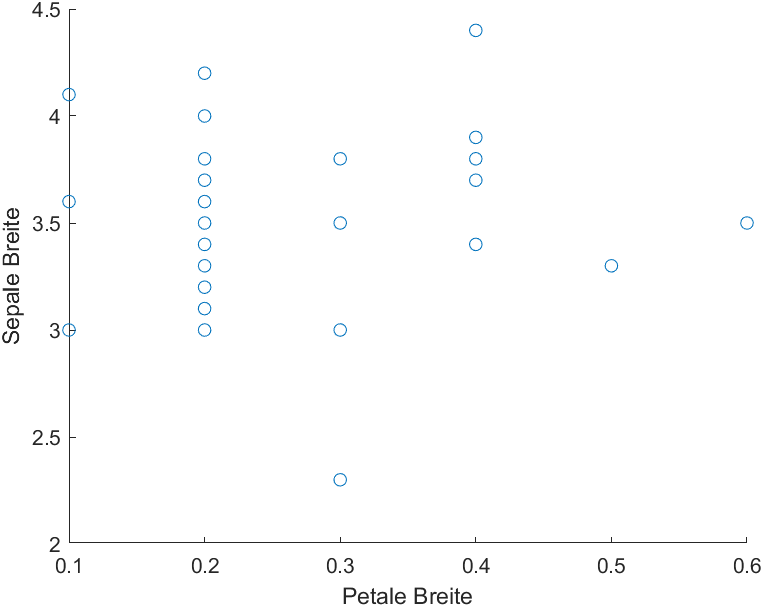
\includegraphics[width=0.7\linewidth]{assignment2_data/plots/4fi}
		\item Petale Länge und sepale Länge scheinen ebenfalls unkorreliert zu sein.\\ 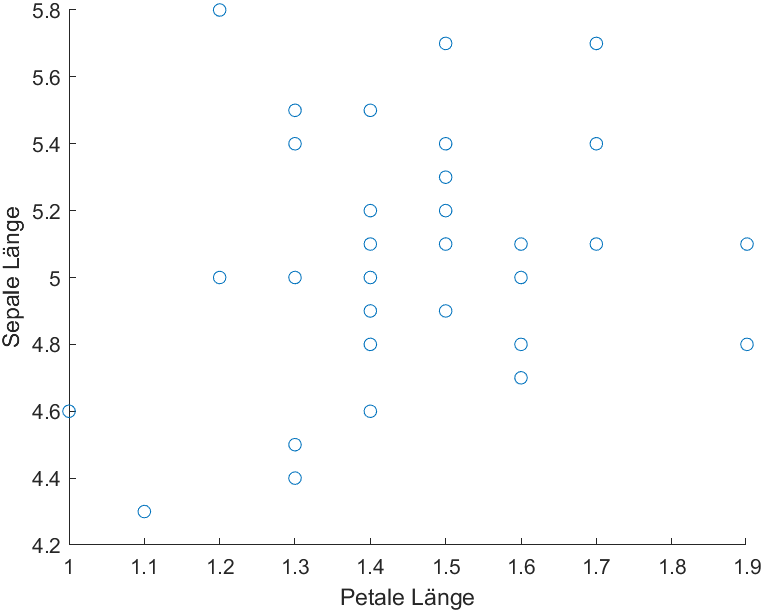
\includegraphics[width=0.7\linewidth]{assignment2_data/plots/4fii}
		\item Zwischen Petaler Länge und petaler Breite scheint ein leichter Zusammenhang zu bestehen, d.h. wenn die petale Länge größer ist, ist oft auch die petale Breite größer.\\ 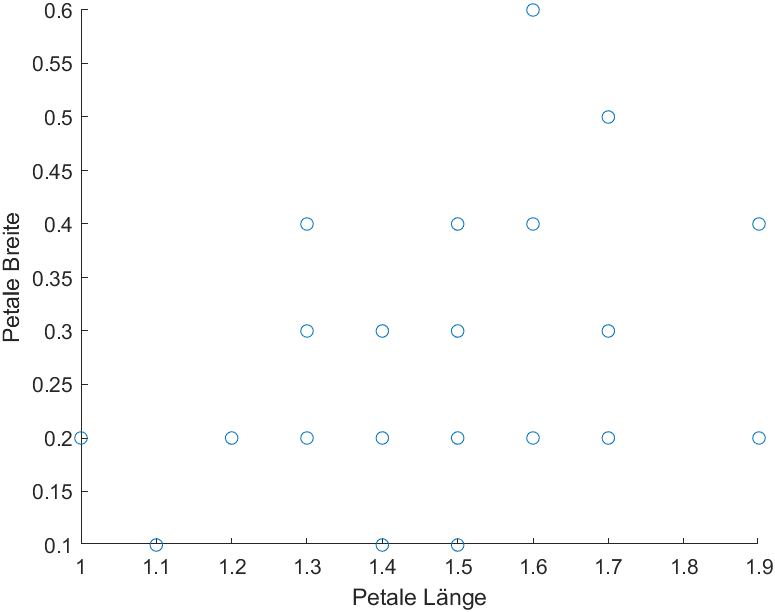
\includegraphics[width=0.7\linewidth]{assignment2_data/plots/4fiii}
		\item Zwischen sepaler Länge und sepaler Breite besteht ein klarer Zusammenhang. Ist die sepale Länge groß, so ist die sepale Breite ebenfalls groß.\\  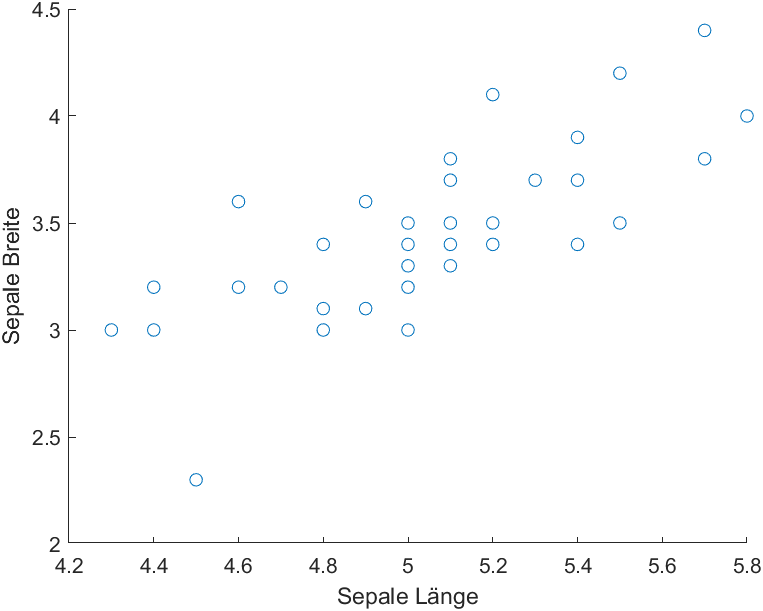
\includegraphics[width=0.7\linewidth]{assignment2_data/plots/4fiv}
	\end{itemize}
	\item[g)] Der einzige Unterschied in der Klassifikation besteht darin, dass diesmal alle Datenpunkte richtig klassifiziert wurden. 
	%TODO Beispielplot

\end{itemize}


\end{document}